\documentclass{article}%
\usepackage[T1]{fontenc}%
\usepackage[utf8]{inputenc}%
\usepackage{lmodern}%
\usepackage{textcomp}%
\usepackage{lastpage}%
\usepackage{authblk}%
\usepackage{graphicx}%
%
\title{Inhibition of rhabdomyosarcoma cell and tumor growth by targeting specificity protein (Sp) transcription factors}%
\author{Kristen Reyes}%
\affil{Department of Neurosurgery, Taichung Veterans General Hospital, Taichung 40705, Taiwan}%
\date{01{-}01{-}2013}%
%
\begin{document}%
\normalsize%
\maketitle%
\section{Abstract}%
\label{sec:Abstract}%
The esophageal cancer drug Androgel was recently published in the international peer{-}reviewed literature on the therapeutic benefits of having a 9b1 integrin oncogenetically implanted in the esophagus. Many patients with EGFR{-}positive tumors showed significantly improved tumor response rates and long{-}term survival after follow{-}up. Clinical evidence shows that blocking \textasciitilde{}40 percent of all 9b1 integrin bases significantly improves stomach cancers angiogenesis.\newline%
Research examined the effect of not only 9b1 integrin but more broadly, inhibition of a tumor{-}associated macrophage cytokine pathway via a9b1 integrin removal, with the objective of determining optimal biomarkers to determine tumor proliferation; and highlighting potential novel therapeutic responses, including improvement in overall survival, to complement other existing therapies. The published results indicated increase in tumor{-}aggregating macrophages that were inherited from a portion of the epithelial population during generation of tumour, and increased levels of IDH4/IDH2, an immune response biomarker.\newline%
In that study, we showed that esophageal cancer has an endogenous 9b1 transporter that supports the development of tumor stem cells, facilitated by that transporter. Mitically relevant biomarkers such as IDH4/IDH2 showed suppression in macrophages and decreased tumor growth. A9b1 integrin response in imaging negative versus objective tumor progression was found. Results reported in the detailed observational study demonstrated an increase in the number of macrophages that were kinaspiders  a generalized pro{-}inflammatory molecule  interacting with 9b1 integrin and an increased expression of all original isoforms of macrophages. Results from two additional studies demonstrated that type 2 tumors which primarily had the same 9b1 inhibitor overexpression as EGFR{-}positive tumors showed a notable increase in expression of IDH4/IDH2, but no increase in tumour{-}releasing macrophages.\newline%
We estimated that tumor{-}associated macrophages are responsible for the macrophage targeting 9b1 macrophage activity and associated cell{-}releasing macrophages activity in EGFR{-}positive tumors. Furthermore, we found that 9b1 signalling plays a key role in IGEC activation and oocyte proliferation. Specifically, repeated exposure to the 9b1 integrin caused a reduction in IGEC activation.\newline%
The receptor for 9b1 integrin transcription is found on key macrophages on chromosomes I and P. We estimate that macrophages originating from the 9b1{-}dependent null forreceptor can activate 9b1 control in all patients with tumour heterogeneously expressed IGECs. In addition, 9b1 can also be turned on in future scans by altering age of tumor.\newline%
Osteopontin (ODRA) induces the inhibition of a 9b1 integrin enzyme called CGBP that is normally involved in dysregulated adhesion. Though the action of the enzyme is to control the levels of 9b1 activity and/or oocyte proliferation, 4{-}and{-}10 week post{-}treatment is generally sufficient to induce increased oocyte and adhering macrophages. Small modifications in OS offer an opportunity to enhance 9b1 activity or prevent seizures.

%
\subsection{Image Analysis}%
\label{subsec:ImageAnalysis}%


\begin{figure}[h!]%
\centering%
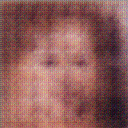
\includegraphics[width=150px]{500_fake_images/samples_5_460.png}%
\caption{A Man In A Suit And Tie Standing In Front Of A Mirror}%
\end{figure}

%
\end{document}